\section{Fixing the Compilation of the Contract}\label{sec:fix}

The security issue in Sec.~\ref{sec:attack} is due to the
over-permissive erasure of the signature of method \<accept>,
where the compiler gives \<buyer> the type \<PayableContract>.
Therefore, a solution is to oblige the compiler to generate a more
restrictive signature where, in particular, the parameter \<buyer>
has type \<TendermintED25519Validator>: only that type of accounts
must be accepted for the validators, consequently banning instances of \<Attacker>.

\begin{figure}[ht]
  \begin{center}
    \begin{lstlisting}[language=Takamaka]
public class TendermintValidators
   extends AbstractValidators<TendermintED25519Validator> {

  public TendermintValidators(TendermintED25519validator validator, BigInteger power) {
    super(validator, power);
  }

  @Override @FromContract(PayableContract.class) @Payable
  public void accept
    (BigInteger amount, TendermintED25519Validator buyer, 
     Offer<TendermintED25519Validator> offer) {
    super.accept(amount, buyer, offer);
  }
}
    \end{lstlisting}
  \end{center}
  \caption{The fixed code of the shared entity of the validators of a Hotmoka blockchain built over Tendermint.}\label{fig:solution}
\end{figure}

The fixed code is shown in Fig.~\ref{fig:solution}. The only difference is that method
\<accept> has been redefined to enforce the correct type for \<buyer>
(see that redefined method also in Fig.~\ref{fig:hierarchy-entities}). For the rest, that method
delegates to its implementation inherited from \<AbstractValidators>, through a call
to \<super.accept>.
It is important to investigate which is the Java bytecode generated from
the code in Fig.~\ref{fig:solution}. Since Java bytecode does not allow one to redefine a method
and modify its argument types, the compiled bytecode actually contains \emph{two}
\<accept> methods, as follows:

\begin{lstlisting}[language=JavaBytecode]
public class TendermintValidators extends AbstractValidators {
  ...
  
  public void accept(BigInteger,TendermintED25519Validator,Offer)
   aload_0
   aload_1
   aload_2
   aload_3
   invokespecial AbstractValidators.accept
                        (BigInteger,PayableContract,Offer)
   return

  // synthetic bridge method
  public void accept(BigInteger,PayableContract,Offer)
   aload_0
   aload_1
   aload_2
   checkcast TendermintED25519Validator
   aload_3
   invokevirtual accept(BigInteger,TendermintED25519Validator,Offer)
   return
}
\end{lstlisting}

\noindent
The first \<accept> method above is the compilation of that from Fig.~\ref{fig:solution}:
it delegates to the \<accept> method of the superclass \<AbstractValidators>. The second
\<accept> method above is a \emph{bridge method} that the compiler generates in order to guarantee
that all calls to the erased signature \<accept(BigInteger,PayableContract,Offer)> actually
get forwarded to the first, redefined \<accept>. It casts its \<buyer> argument
into \<TendermintED25519Validator> and calls the first \<accept>. This
bridge method and its checked cast guarantee that only \<TendermintED25519Validator>s
can become validators. As shown in Fig.~\ref{figure.solution},
an instance of \<Attacker> (Fig.~\ref{fig:attacker})
cannot be passed to the first \<accept> (type mismatch) and makes the second \<accept>
fail with a class cast exception. The \emph{Consistency of Shareholders} holds
for instances of \<TendermintValidators> now and the attack in Sec.~\ref{sec:attack} cannot occur
anymore.

The solution of redefining method \<accept> can be seen as a limited form of heterogeneous
compilation of generics, restricted to a specific method and forced manually.
It is interesting to consider which methods
would need that redefinition, in general. They are those that have a parameter of a generic type
that is restricted in a subclass. For instance, method \<accept> in
Fig.~\ref{fig:shared_entity} has parameters \<buyer> and \<offer> of generic type
\<S> and \<O>, respectively. The subclass in Fig.~\ref{fig:validators} restricts
\<S> to be a \<TendermintED25519Validator> and \<O> to be
an {\codesize\texttt{Offer<TendermintED25519Validator>}}. Hence we must redefine
\<accept> in the subclass with the more specific types for the \<buyer> and \<offer>
parameters. In the future, a compiler might perform this automatically or a static analysis
tool might issue a warning when such redefinition is needed. Currently, however, that is
left to the programmer of the smart contracts, who might overlook the problem
and give rise to security issues, as shown in Sec.~\ref{sec:attack}.

\begin{figure}[ht]
\centering
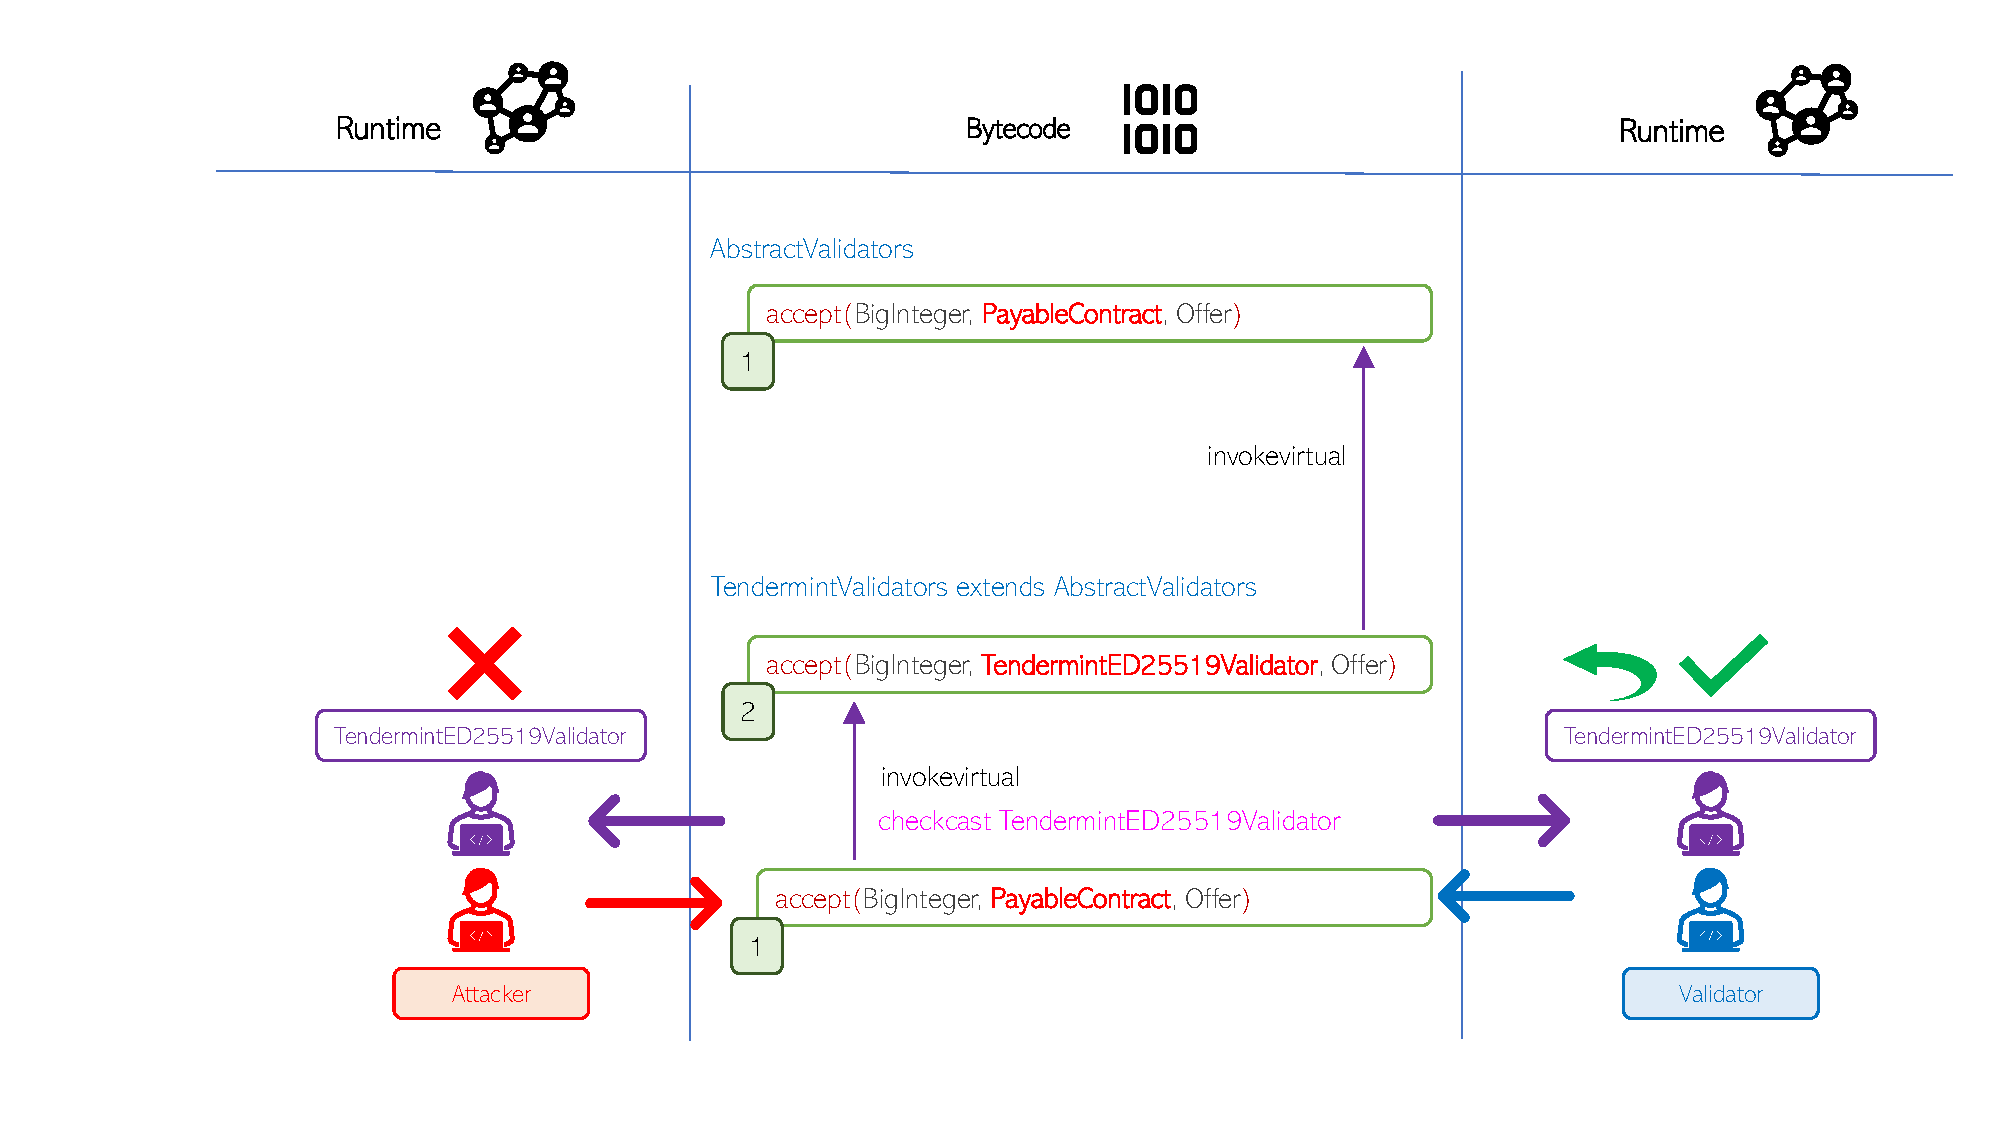
\includegraphics[width=.95\linewidth]{figures/solution}
\caption{Example of how the proposed solution works at run time when the \<accept> method is called by a \<Validator> or an \<Attacker>.}
\label{figure.solution}
\end{figure}

